\documentclass[11pt, letterpaper, twoside]{article}
\usepackage[utf8]{inputenc}
\usepackage[T1]{fontenc}
\usepackage{fancyhdr}
\usepackage[margin=1in, include foot]{geometry}
\usepackage{ragged2e}
\usepackage[hidelinks]{hyperref}
\usepackage{apacite}
\usepackage{setspace}
\usepackage{caption}
\usepackage{subcaption}
\usepackage{etoolbox}
\usepackage{graphicx}
\usepackage{amsmath}
\usepackage{cleveref}
\usepackage{wrapfig}
\usepackage{afterpage}
\usepackage{floatrow}
\usepackage{tikz}

\setlength\parindent{0pt}

\title{\singlespacing\textbf{DOCUMENTATION FOR: ``Getting as good as you give: The effects of the press on politician's post-office earnings''}}

\author{Joshua Y. Levy \thanks{Joshua Y. Levy  (joshua.levy@chicagobooth.edu), Stigler Center, Booth School of Business, University of Chicago}}
\date{\today}


\begin{document}
\begin{titlepage}
    \maketitle
    \thispagestyle{empty}
\end{titlepage}


\newpage
\pagenumbering{arabic}

\textsc{\textbf{hypothesis: }}Corporations have a continued interest in accessing the halls of power to better navigate the law to their own ends. Thus, a so-called ``revolving door'' effect has emerged whereby government officials begin working for -- or at the behest of -- private corporations shortly after leaving office to help their new masters/clients navigate, shape, and benefit from rules, regulations, and laws. We suppose however, that a business is willing to retain a former government official or leader, conditional on the leader's competence and/or ideological leanings. Despite often maintaining large government relations departments, we suppose that business leaders are sensitive to the signals of leaders' competence (and pro-business attitudes) issued by elite, business-facing news publications such as \textit{The Economist}. That is, we hypothesize that the more favorably such publications write about a leader, the more they are likely to earn as consultants to, or employees of private corporations after leaving office.\\

Enclosed is documentation about the methodology and some preliminary results working to verify this hypothesis.

\section{00 - The Economist Scraper}

In order to test this hypothesis, I begin by collecting the corpus of \textit{The Economist}. I use a Python script to scrape all articles stored by ProQuest: ABI/Inform.\footnote{\textbf{N.B.} Apparently this violates UChicago library policy. Please continue reading for information on collection.} Comments are included on each script but below is a high-level overview of this step's organization. The bulleted list is in order that each script should be run. The key output file of this folder is ``formatted\_compiled\_articles.csv'' which is a three column .csv file with the headers: ``date,'' ``link,'' and ``text'' containing the date of the issue the article was published in, the link to the ABI/Inform page from which the text was scraped, and the body of the text, respectively. This script collects on the order of 123,000 articles between January 1992 and December 2019.

\begin{itemize}
    \item \textbf{ABI-INFORM Economist Scraper.py}\\
    This Python script that does the bulk of the article collection. It is broken into two parts: (1) visiting ``issue-level'' pages to collect links to every article; and (2) visiting every ``article-level'' page (links to which were collected in part (1)) to collect the body of each article's text. There are a number of parameters that need to be set by the user to run this script correctly describe in the commented header.\\
    
    Note that this scraper was written to access a database that sits behind shibboleth-style dual-factor authentication (specifically the University of Chicago's). As a result, it requires some amount of supervision to run properly. If just part (1) is run then the only supervision required is at the time of initiating the scraper as the user must create an authenticated session which a Selenium driver will use to collect links to articles. (Note that Selenium is used in part (1) because the issue-level pages interact with the server using AJAX so the page is dynamic and the scraper must wait for certain information to load into the page before parsing the HTML.)\\

    If just part (2) is run then the user is required to supervise somewhat more closely. As before, the user will have to authenticate their session to generate a set of authenticated cookies that will be used by the article-level scraper. This secondary article-scraper runs using the requests library in Python because it is faster than simulating the entire browser experience (as Selenium does). However, dynamically updating the authenticated cookies so that the authenticated session does not time out becomes prohibitively difficult. Instead, a single authenticated cookie is passed to each request which generates a new session. By my experimentation, it is thus best to run the scraper 10,000 requests (i.e 10 ``batches'' of a thousand requests each) at a time. This maximizes scraping for minimal user re-authentication. Part (2) of the scraper stores links-to and article-text in .csv files of 1,000 rows and saves them to the ``sub\_csvs'' folder as .csv files. Additionally, it generates and updates the ``tracker\_sheet.csv'' file so that successive runs do not generate duplicate article-observations.\\

    \textbf{N.B.} I do NOT recommend running this script again. Bulk collection is in violation of University Library policy and I (Joshua) have already been warned once. We currently have around 1,500 observations that failed and I will collect by hand.
    \item \textbf{csv\_compiler.py}\\
    This Python script reads in each of the .csv files generated by part (2) of the above scraper cleans them. Every quarter \textit{The Economist} produces a ``special report'' consisting of several articles. However, instead of creating separate article-pages for each of these, ABI/Inform collates all of them and saves them on a single page. This results in a very long string that breaks the formatting of the above scraper. This script reformats all of the sub\_csv files and compiles them into a single .csv file that can be used for subsequent analysis. The output of this script is called ``formatted\_compiled\_articles.csv''
\end{itemize}



\section{01 - Leader Selection}

In order to better understand the role that the (business-facing) press has in mediating the sums of money that business pay former leaders for advice or access, we additional narrow the scope of nations under consideration to substantive democracies. I do so for two reasons: first, substantive democracies tend to be more transparent -- suggesting that the press has a bigger role in those nations relative to more autocratic ones. Indeed, in many settings, freedom of the press is considered one of the necessary constituent parts of substantive democracy. Additionally, when considering former leaders of autocratic nations, businesses may be inclined to access or retain former leaders not because of the supposed competence of the leader in question as conveyed by the press, but because of the perception that doing so is either necessary or advantageous for practicing some kind of (illicit) corruption. This thus circumvents the mechanism of interest.\\

What follows is a description of how nations were selected and nations identified.

\begin{itemize}
    \item \textbf{LeaderSelection.R}\\
    This R script identifies nations of interest using the Polity V dataset. Polity constructs a ``score'' at the nation-year level ranging from -10 (most autocratic) to 10 (most democratic). To identify as large a sample of substantive democracies as possible, we identify nation-years that receive a Polity score greater than or equal to 8.\footnote{Note that this level was selected arbitrarily and can be amended.} In order to keep the sample of nations as large as possible, if a nation receives a Polity score of 7 at any point in the sample, but maintains a score of at least 8 for at least 10 years, the country is retained in the sample. This dataset of sample-years is then matched with the REIGN dataset of leader observations.\\

    I additionally use this dataset of leader-years to output two .csv files. The first, ``leaders\_names\_pre\_styling.csv'' is a list of leaders and nations with their REIGN stylings.\footnote{Note that because the REIGN dataset does not include leaders from Taiwan or Montenegro, these are added manually.} This however, is not necessarily how \textit{The Economist} styles the leaders names. I modify this list, identifying \textit{The Economist's} editorial style saving it ``leaders\_names\_econ\_styling.csv''. A similar process is conducted for ``countries\_pre\_details.csv''. This .csv simply contains a list of countries of interest. I then add nation-level information such as the leader's title (e.g. prime minister, president, chancellor, etc.) national denonyms (e.g. Chileans, Japanese, etc.) and other information. This is stored in ``national\_titles\_adjectives.csv''. These files are important for cleanly identifying leaders within the body of text of each article.
\end{itemize}

\begin{table}[ht]
    \centering
    \small{\textbf{Table 1:} Summary Statistics}
    \begin{tabular}{rlll}
      \hline
     &   country &     polity &      year \\ 
      \hline
     & Length:1952        & Min.   : 7.00   & Min.   :1992   \\ 
     & Class :character   & 1st Qu.: 8.00   & 1st Qu.:2001   \\ 
     & Mode  :character   & Median : 9.00   & Median :2007   \\ 
     &  & Mean   : 9.19   & Mean   :2007   \\ 
     &  & 3rd Qu.:10.00   & 3rd Qu.:2013   \\ 
     &  & Max.   :10.00   & Max.   :2019   \\ 
       \hline
    \end{tabular}
\end{table}


\section{02 - Coreference Resolution}
Coreference resolution is a natural language process (NLP) technique by which ambiguous noun-phrases or ``entities'' within a body of text are identified and ``resolved'' to be unambiguous. For instance, the following text remains semantically ambiguous to a computer. ``The quick brown box jumped over the lazy dog. It flew through the air.'' The pronoun, ``it,'' at the beginning of the sentence clearly refers to the ``fox'' in the first sentence, but a computer is regularly unable to discriminate between this potential relationship and a potential relationship between ``it'' and the ``dog''\\

To mitigate this problem I use a combination of NLP tools: Allen NLP's pre-trained SpanBERT Coreference resolution model and spacy, a general purpose NLP tool \cite{Lee2018HigherorderCR}. Trained on hundreds of thousands of sentences that have been marked for their semantic and lexicographic features such as part of speech, position relative to punctuation, subject-object relationship, number consistency, etc. SpanBERT  can resolve the above example to: ``The quick brown fox jumped over the lazy dog. The fox flew through the air.''\\

This process is important because SentimentR (described in greater detail below) assesses sentiment at the sentence-level. Thus, it is important for us to maximize the sample of sentences that semantically refer to our entities of interest: former leaders. For example on January 23rd, 1991, \textit{The Economist} published an article that began as follows:
\begin{quote}
    ``The one thing his aides had told him to do was to keep it brief and for once he listened. On January 20th, moments after being sworn in as America's 42nd president, Bill Clinton gave an inaugural address that clocked in at under 15 minutes.''
\end{quote}
Naively passing these two sentences for sentiment analysis would yield only one observation of a Clinton-sentence. However, using coreference resolution, I resolve this text to:
\begin{quote}
    ``The one thing Bill Clinton's aides had told Bill Clinton to do was to keep it brief, and for once Bill Clinton listened. On January 20th, moments after being sworn in as America's 42nd president, Bill Clinton gave an inaugural address that clocked in at under 15 minutes.''
\end{quote}
Because the corpus of \textit{The Economist} contains many more non-leader sentences than it does leader sentences, maximizing the number of semantic signals for sentiment analysis is of the utmost importance.

\begin{itemize}
    \item \textbf{coref\_resolver.py}\\
    This Python script completes several tasks. First it creates an index file, ``date\_index.csv'' so that it is not necessary to keep all 123,000+ articles in memory at any given time. This script additionally reads in leader-level information from ``leader\_meta\_matched.csv'' so that it is possible to create a subset of potential articles to search on. It then reads in all articles published six months before, during, and six months after the term of the leader of interest. The script then tags the articles which contain a mention of a leader so that coreferences can be resolved. This script generates a series of .csv files as outputs, one for each leader and stores them in the ``leader\_tagged\_resolved'' folder with the format ``[LEADERLASTNAME]\_[COUNTRYCODE]\_resolved.csv'' \textbf{NOTE:} Coreference is a computationally expensive task. DO NOT RUN THIS FILE WITHOUT THINKING ABOUT SAMPLE SIZES. Each such .csv file contains article meta-data, the original article text, and the resolved text.\\
\end{itemize}


\section{03 - Sentiment Analysis}
To test our hypothesis, it is necessary to have a systematic way by which to evaluate the way\textit{The Economist} writes about (various) leaders, and indeed if there exists considerable hetereogeneity in its editorial position on each leader's performance. That is, we need a way to consistently measure if \textit{The Economists} writes more favorably of some leaders than it does others.\\

The tool that I use, an R package called SentimentR, attempts to do this by using an ``augmented dictionary approach.'' \cite{rinker2019sentimentr} The most simple way to measure sentiment is to first construct a dictionary of ``positive'' and ``negative'' words, and then simply tally up the number of times such words appear in a body of text. One could additionally, weight some words more heavily than others --- ``exemplary,'' for example might receive a stronger positive weighting than ``fair.''\\

SentimentR introduces another layer of complexity by identifying ``valence shifters,'' that may amplify, mitigate, or completely alter the sentiment of a cluster of positive or negative words. After identifying ``polarity clusters,'' the SentmentR algorithm alters a sentence's score based on the presence or absence of these shifters. Words like ``however,'' ``but,'' and ``although,'' for example, are adversative conjunctions that can amplify or de-amplify a cluster's polarity based on their position in the sentence relative to the cluster.\\

SentimentR conducts analysis at the sentence-level. Thus, as noted above, maximizing the number of sentences that mention a leader is important because an article's latent information about a leader's competence can easily be identified by a human reader but not by a computer.\\

Below is an example of SentimentR output based on 79 articles worth of text. Each point represents a sentence observation. The imposed line is Lowess-smoothed line of average sentiment at each date of observation (issue publication date). Note that though sentiment generally ranges from -1, the most negative, to 1, the most positive, valence shifters can give a sentence a score beyond these bounds. The entire sample of sentences are from articles that mention ``Obuchi'' (or one of the appropriate aliases). \\


\newpage
\begin{figure}
    \centering
    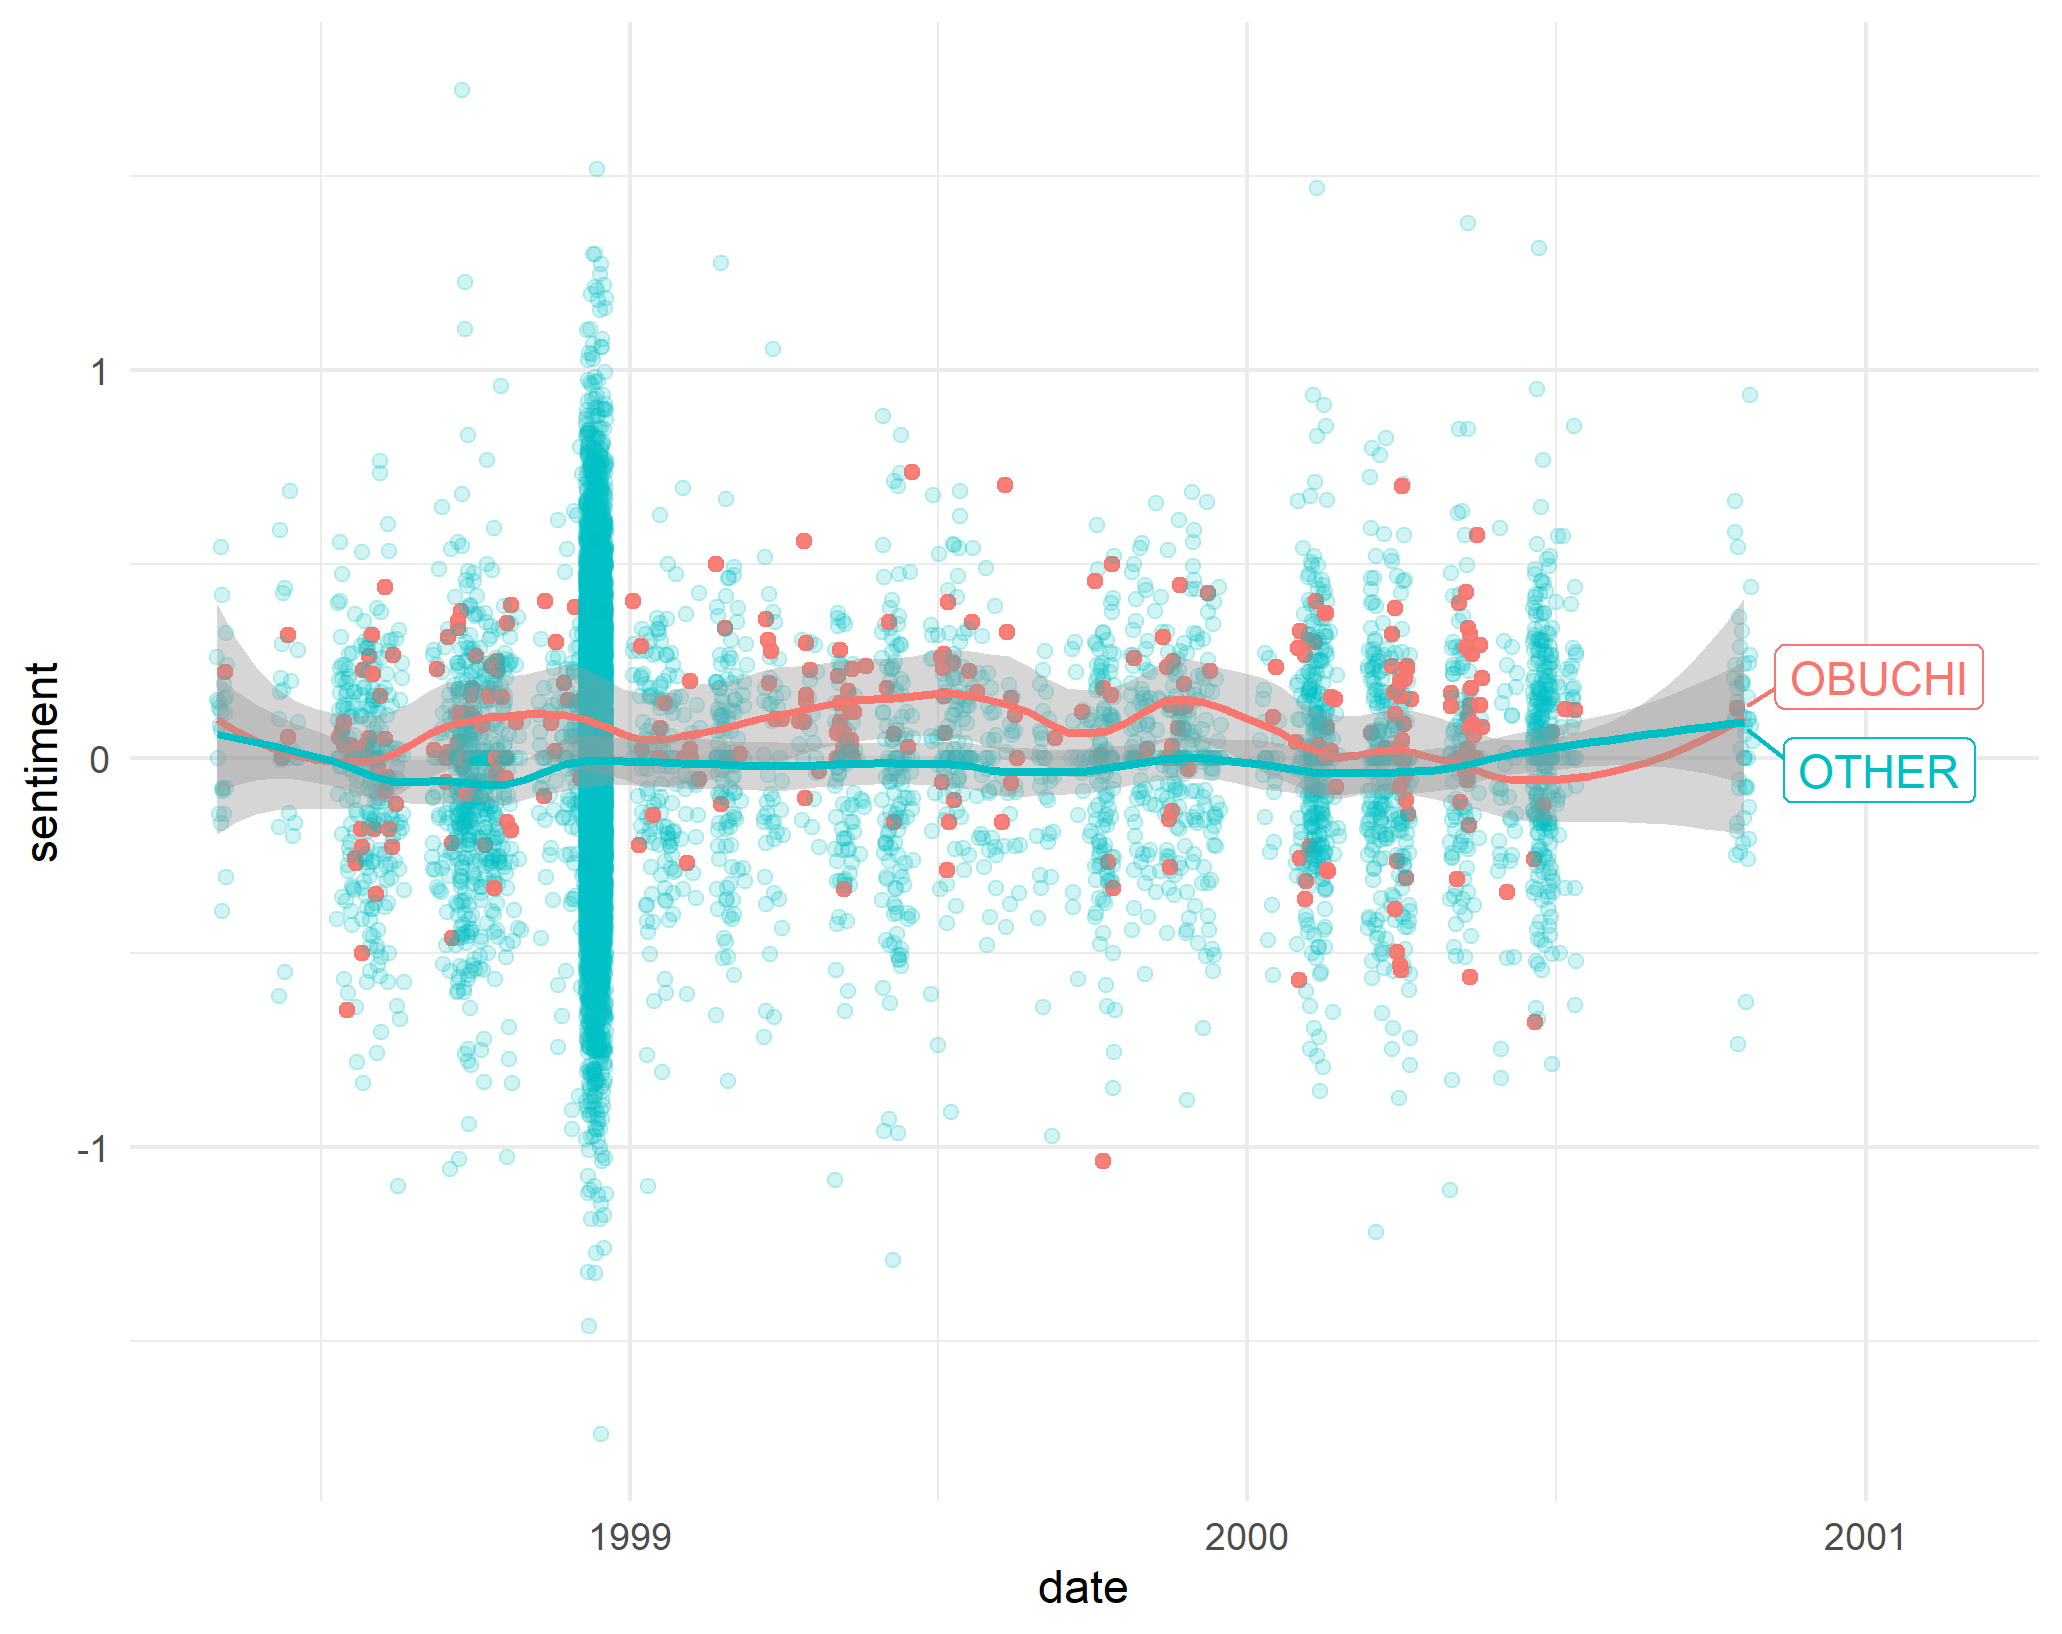
\includegraphics[clip, width=0.8\textwidth]{figures/obuchi_sentiment_time.png}
    \caption{Average sentiment of ``Obuchi'' sentences over time}
\end{figure}

% \begin{table}[ht]
%     \small{\textbf{Table 2:} SentimentR Results for Articles Containing ``Clinton''}
%     \centering
%     \begin{tabular}{rlrrr}
%       \hline
%      & Sentence Type & Word Count & SD & Mean Sentiment \\ 
%       \hline
%     1 & CLINTON & 1277 & 0.25 & 0.0125 \\ 
%       2 & OTHER & 3490 & 0.30 & -0.0127 \\ 
%        \hline
%     \end{tabular}
% \end{table}

% \vspace{0.2\textwidth}


\section{04 - Officer Pay}
There is large variation in the official pay for world leaders. In addition to receiving a public salary, leaders may additionally be entitled to ``fringe benefits'' such as accommodation (in a Presidential Palace or Residence, for example) free travel when on official business, and other forms of non-pecuniary remuneration. Because it is hard to calculate the true value of these benefits, I limit definitions of compensation to salaried pay.\\

Below is a sample of OECD nation's leaders and their pay. (Note that this is an incomplete sample because of disagreements between whether the ``head of government'' or ``head of state'' is the true chief executive of a country. Take, for example, the conflict of such status in France where the head of state, President Emmanuel Macron, is the chief executive. His counterpart in the UK however, is prime minister Boris Johnson, the head of government.)

\begin{figure}
    \centering
    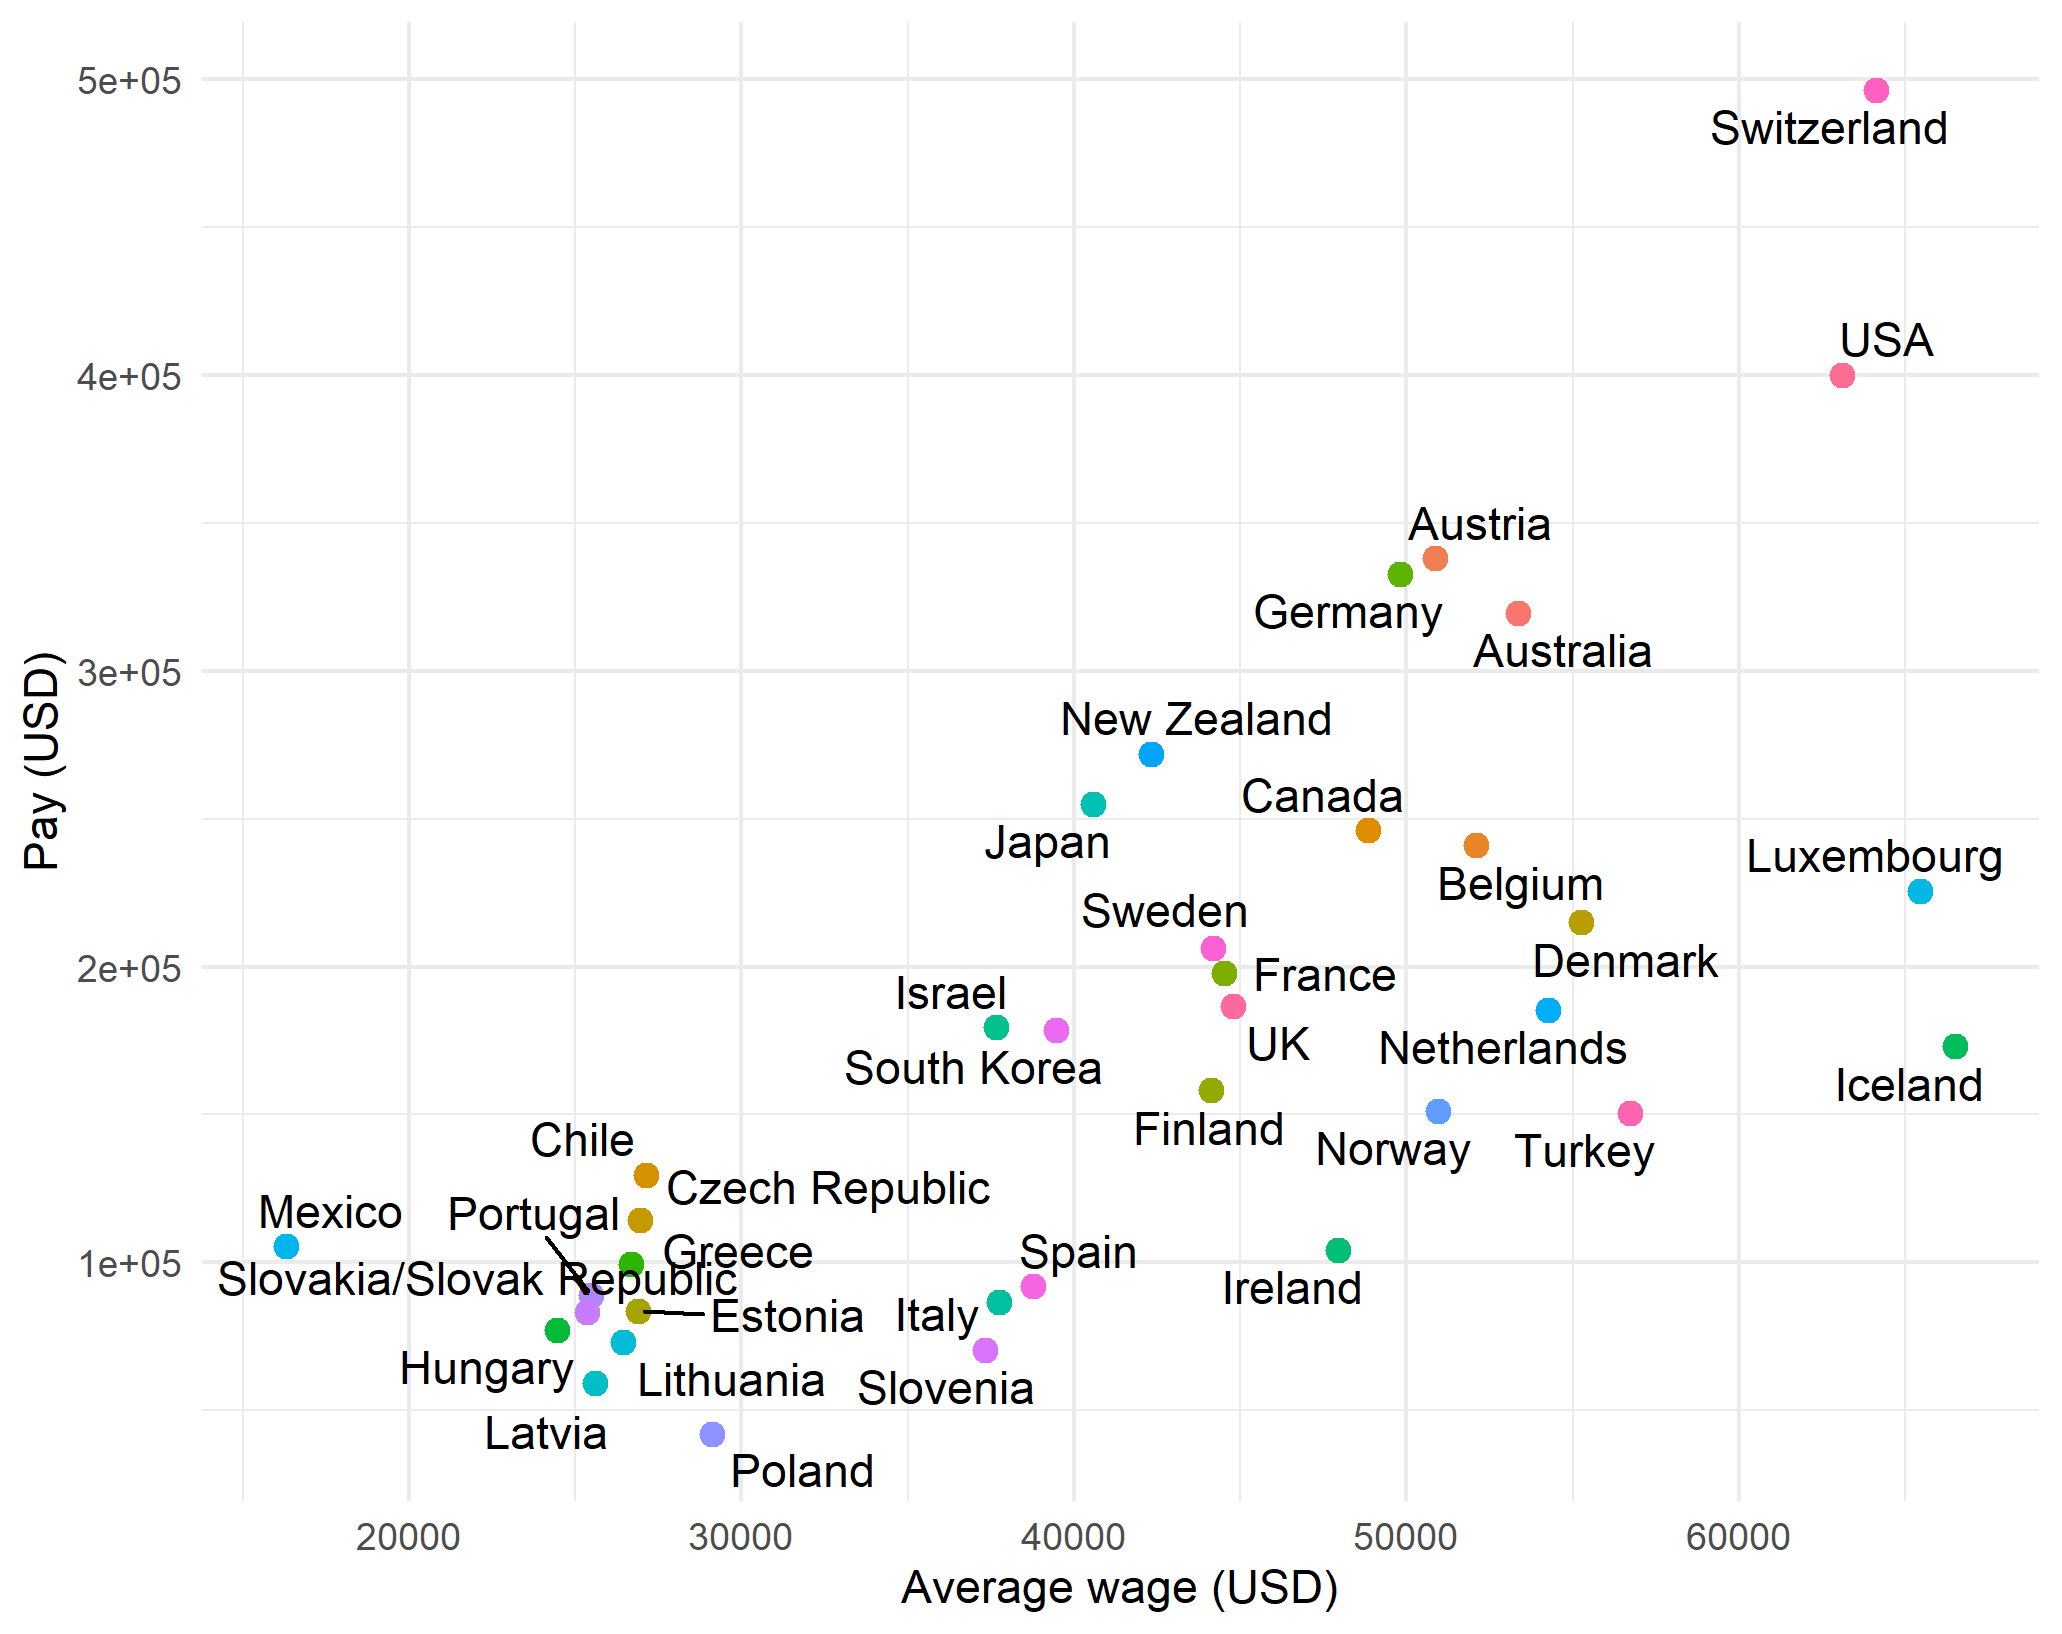
\includegraphics[clip, width=0.8\textwidth]{figures/leader_pay.png}

\end{figure}





\nocite{bell2016rulers}
\newpage
\bibliographystyle{apacite}
\bibliography{readmebib}
\newpage

\end{document}
